% Options for packages loaded elsewhere
\PassOptionsToPackage{unicode}{hyperref}
\PassOptionsToPackage{hyphens}{url}
%
\documentclass[
  11pt,
  a4paper,
]{article}
\usepackage{amsmath,amssymb}
\usepackage{lmodern}
\usepackage{iftex}
\ifPDFTeX
  \usepackage[T1]{fontenc}
  \usepackage[utf8]{inputenc}
  \usepackage{textcomp} % provide euro and other symbols
\else % if luatex or xetex
  \ifXeTeX
    \usepackage{zxjatype} 
    \usepackage[ipaex]{zxjafont}
    \setromanfont{Times New Roman}
  \fi
  \usepackage{unicode-math}
  \defaultfontfeatures{Scale=MatchLowercase}
  \defaultfontfeatures[\rmfamily]{Ligatures=TeX,Scale=1}
\fi
% Use upquote if available, for straight quotes in verbatim environments
\IfFileExists{upquote.sty}{\usepackage{upquote}}{}
\IfFileExists{microtype.sty}{% use microtype if available
  \usepackage[]{microtype}
  \UseMicrotypeSet[protrusion]{basicmath} % disable protrusion for tt fonts
}{}
\usepackage{xcolor}
\IfFileExists{xurl.sty}{\usepackage{xurl}}{} % add URL line breaks if available
\IfFileExists{bookmark.sty}{\usepackage{bookmark}}{\usepackage{hyperref}}
\hypersetup{
  pdftitle={Draft of Data and Estimation Result},
  hidelinks,
  pdfcreator={LaTeX via pandoc}}
\urlstyle{same} % disable monospaced font for URLs
\usepackage[left=3cm,right=3cm,top=3cm,bottom=3cm]{geometry}

\usepackage{setspace}
\renewcommand{\baselinestretch}{1.5}
\usepackage{float}

\usepackage{longtable,booktabs,array}
\usepackage{threeparttable, threeparttablex, multirow}
\usepackage{calc} % for calculating minipage widths
% Correct order of tables after \paragraph or \subparagraph
\usepackage{etoolbox}
\makeatletter
\patchcmd\longtable{\par}{\if@noskipsec\mbox{}\fi\par}{}{}
\makeatother
% Allow footnotes in longtable head/foot
\IfFileExists{footnotehyper.sty}{\usepackage{footnotehyper}}{\usepackage{footnote}}
\makesavenoteenv{longtable}
\usepackage{graphicx}
\makeatletter
\def\maxwidth{\ifdim\Gin@nat@width>\linewidth\linewidth\else\Gin@nat@width\fi}
\def\maxheight{\ifdim\Gin@nat@height>\textheight\textheight\else\Gin@nat@height\fi}
\makeatother
% Scale images if necessary, so that they will not overflow the page
% margins by default, and it is still possible to overwrite the defaults
% using explicit options in \includegraphics[width, height, ...]{}
\setkeys{Gin}{width=\maxwidth,height=\maxheight,keepaspectratio}
% Set default figure placement to htbp
\makeatletter
\def\fps@figure{htbp}
\makeatother
\setlength{\emergencystretch}{3em} % prevent overfull lines
\providecommand{\tightlist}{%
  \setlength{\itemsep}{0pt}\setlength{\parskip}{0pt}}
\setcounter{secnumdepth}{5}
\newlength{\cslhangindent}
\setlength{\cslhangindent}{1.5em}
\newlength{\csllabelwidth}
\setlength{\csllabelwidth}{3em}
\newlength{\cslentryspacingunit} % times entry-spacing
\setlength{\cslentryspacingunit}{\parskip}
\newenvironment{CSLReferences}[2] % #1 hanging-ident, #2 entry spacing
 {% don't indent paragraphs
  \setlength{\parindent}{0pt}
  % turn on hanging indent if param 1 is 1
  \ifodd #1
  \let\oldpar\par
  \def\par{\hangindent=\cslhangindent\oldpar}
  \fi
  % set entry spacing
  \setlength{\parskip}{#2\cslentryspacingunit}
 }%
 {}
\usepackage{calc}
\newcommand{\CSLBlock}[1]{#1\hfill\break}
\newcommand{\CSLLeftMargin}[1]{\parbox[t]{\csllabelwidth}{#1}}
\newcommand{\CSLRightInline}[1]{\parbox[t]{\linewidth - \csllabelwidth}{#1}\break}
\newcommand{\CSLIndent}[1]{\hspace{\cslhangindent}#1}


\usepackage{booktabs}
\usepackage{longtable}
\usepackage{array}
\usepackage{multirow}
\usepackage{wrapfig}
\usepackage{float}
\usepackage{colortbl}
\usepackage{pdflscape}
\usepackage{tabu}
\usepackage{threeparttable}
\usepackage{threeparttablex}
\usepackage[normalem]{ulem}
\usepackage{makecell}
\usepackage{xcolor}
\usepackage{siunitx}
\newcolumntype{d}{S[input-symbols = ()]}
\ifLuaTeX
  \usepackage{selnolig}  % disable illegal ligatures
\fi

\makeatletter
\def\@fnsymbol#1{\ensuremath{\ifcase#1\or \dagger\or \ddagger\or
   \mathsection\or \mathparagraph\or \|\or **\or \dagger\dagger
   \or \ddagger\ddagger \else\@ctrerr\fi}}
    \makeatother
\title{Draft of Data and Estimation Result  }
\author{
    Hiroki Kato
  \thanks{Graduate School of Economics, Osaka University, Japan. E-mail: vge008kh@stundent.econ.osaka-u.ac.jp  }
  \and
    Tsuyoshi Goto
  \thanks{Graduate School of Social Sciences, Chiba University, Japan. E-mail: t.goto@chiba-u.jp  }
  \and
    Youngrok Kim
  \thanks{Graduate School of Economics, Kobe University, Japan.  }
  \and
  }

\date{2022/04/17}


\begin{document}
\begin{spacing}{1}
  \maketitle
\end{spacing}

\hypertarget{nastab}{%
\section{National Survey of Tax and Benefit (NaSTaB)}\label{nastab}}

本研究は2008年からKorea Institute of Taxation and Financeが実施した
National Survey of Tax and Benefit (NaSTaB)を用いる。
これは家計の税負担や公的扶助などに関する年次パネルデータである。
この調査は全国から5,634世帯を対象とし、
5,634人の世帯主と15歳以上で経済活動をしている世帯員が調査に回答する。
この調査は前年の所得や寄付額に関する情報を含んでおり、
それらに加えて、教育年数などの個人属性や税制に対する個人の意識に関する情報を含んでいる。

\begin{table}

\caption{\label{tab:SummaryCovariate}Descriptive Statistics}
\centering
\fontsize{9}{11}\selectfont
\begin{tabular}[t]{lcccccc}
\toprule
  & N & Mean & Std.Dev. & Min & Median & Max\\
\midrule
\addlinespace[0.3em]
\multicolumn{7}{l}{\textbf{Income and giving price}}\\
\hspace{1em}Annual taxable labor income (unit: 10,000KRW) & 36189 & \num{1747.26} & \num{2696.77} & \num{0.00} & \num{0.00} & \num{50000.00}\\
\hspace{1em}First giving relative price & 36198 & \num{0.86} & \num{0.04} & \num{0.62} & \num{0.85} & \num{0.94}\\
\addlinespace[0.3em]
\multicolumn{7}{l}{\textbf{Charitable giving}}\\
\hspace{1em}Annual chariatable giving (unit: 10,000KRW) & 36199 & \num{35.64} & \num{153.20} & \num{0.00} & \num{0.00} & \num{10000.00}\\
\hspace{1em}Dummary of donation > 0 & 36199 & \num{0.24} & \num{0.42} & \num{0.00} & \num{0.00} & \num{1.00}\\
\hspace{1em}Dummy of declaration of a tax relief & 36199 & \num{0.10} & \num{0.30} & \num{0.00} & \num{0.00} & \num{1.00}\\
\addlinespace[0.3em]
\multicolumn{7}{l}{\textbf{Individual Characteristics}}\\
\hspace{1em}Age & 36199 & \num{53.45} & \num{16.22} & \num{24.00} & \num{51.00} & \num{103.00}\\
\hspace{1em}Female dummy & 36199 & \num{0.43} & \num{0.50} & \num{0.00} & \num{0.00} & \num{1.00}\\
\hspace{1em}University graduate & 36198 & \num{0.42} & \num{0.49} & \num{0.00} & \num{0.00} & \num{1.00}\\
\hspace{1em}High school graduate dummy & 36198 & \num{0.31} & \num{0.46} & \num{0.00} & \num{0.00} & \num{1.00}\\
\hspace{1em}Junior high school graduate dummy & 36198 & \num{0.27} & \num{0.44} & \num{0.00} & \num{0.00} & \num{1.00}\\
\hspace{1em}Wage earner dummy & 27394 & \num{0.56} & \num{0.50} & \num{0.00} & \num{1.00} & \num{1.00}\\
\bottomrule
\end{tabular}
\end{table}

我々の研究では(1)2013年から2018年かつ、(2)23歳以下の回答者を除いたデータを使用する。
データの期間を制限した理由は、2014年の制度改革に注目するためである。
所得控除制度が適用されている期間(2014年の制度改革前)では、所得税率の改正が寄付行動に影響を与える。
この制度が適用されている期間において、所得税率の改正は2011年が最後である。
したがって、2011年以前の寄付行動を用いると、2014年の制度改革以外の影響を含んでしまう。
その可能性を取り除くために、我々は2013年から2018年のデータ(2012年から2017年の寄付行動)を用いる。
また、23歳以下の回答者を除いた理由は、所得や資産を十分に持っていない可能性が高いからである。
表\ref{tab:SummaryCovariate}に記述統計を示した。

\begin{figure}[t]

{\centering 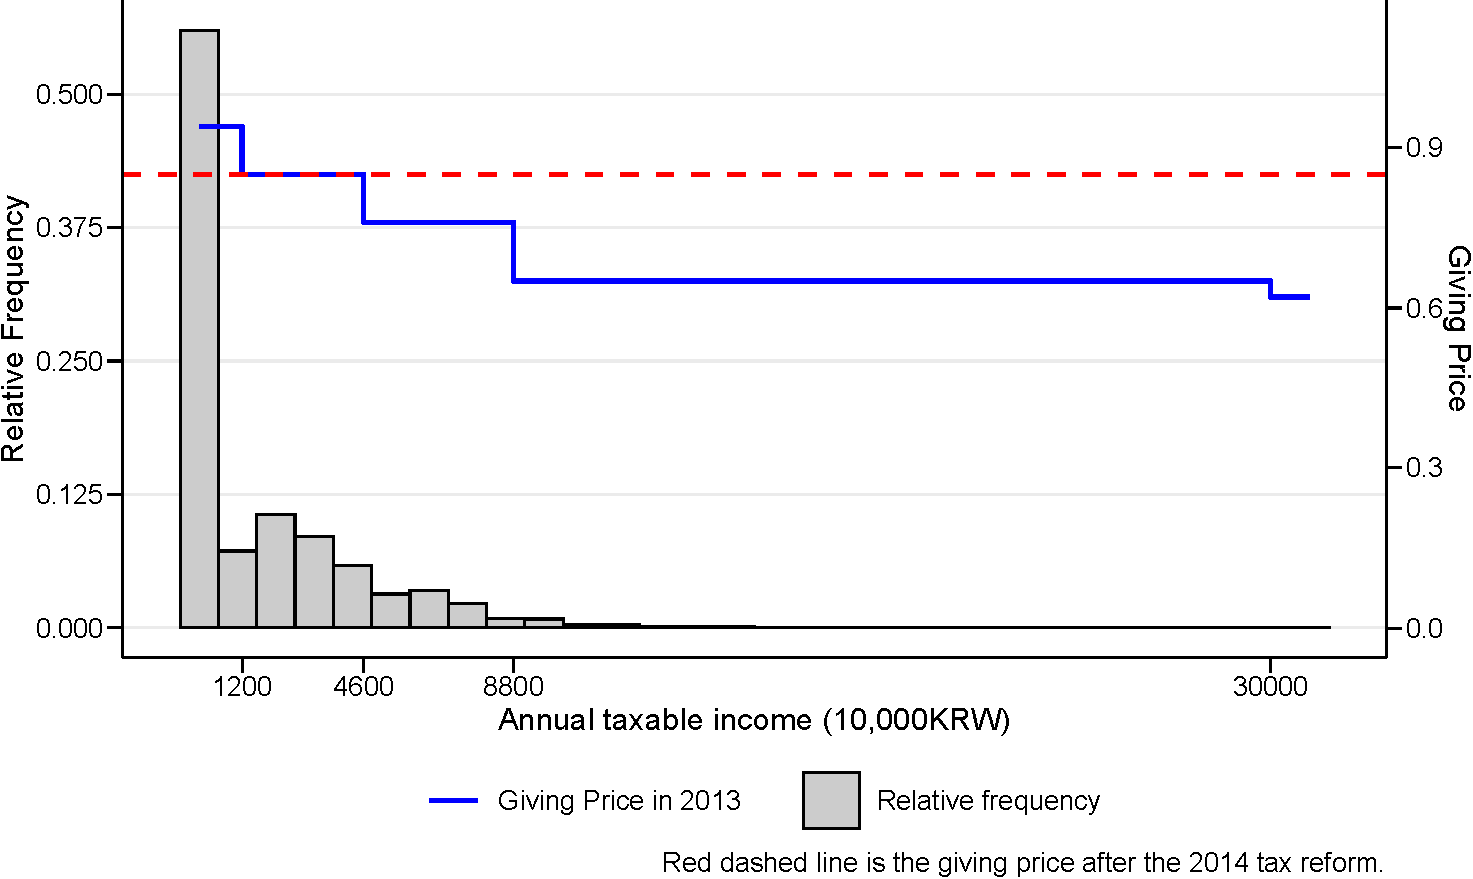
\includegraphics{C:/Users/katoo/Desktop/NASTAB/paper/draft_files/figure-latex/SummaryPrice-1} 

}

\caption{Income Distribution in 2013 and Relative Giving Price. Notes: The left and right axis measure the relative frequency of respondents (grey bars) and the relative giving price (solid step line and dashed line), respectively. A solid step line and a dashed horizontal line represents the giving price in 2013 and 2014, respectively.}\label{fig:SummaryPrice}
\end{figure}

NaSTabは前年の労働所得を調査している。
表\ref{tab:SummaryCovariate}は、
我々が用いるサンプルの労働所得の平均額は17.54 million KRWであることを示しており、
Korean National Tax Serviceが発行しているNational Tax Statistical Yearbook 2012-2018
の平均所得32.77 million KRWより低い。
これはNaSTaBが主婦などの労働所得がない人を含んでいるからである。
したがって、所得分布は右歪曲な分布になる(図\ref{fig:SummaryPrice})。
我々は労働所得に基づいて限界税率を計算し、所得控除における寄付価格を計算した。
図\ref{fig:SummaryPrice}の黒の実線は2012年から2013年の寄付の相対価格を示している。

また、図\ref{fig:SummaryPrice}は価格弾力性を識別するための価格変動も示している。
先に述べたように、黒の実線は所得控除が適用されている期間(2012年から2013年)の寄付の相対価格を示している。
対して、黒の破線は税額控除が適用されている期間(2014年以降)の寄付の相対価格を示している。
2014年の税制改革による税インセンティブの変化に基づいて、我々は三つの所得グループを作ることができる:
(1) 120 million KRWより低い;
(2) 120 million KRWから460 million KRWの間;
(3) 460 million KRWより高い。
第一のグループに属する人の税インセンティブは税制改革によって拡大した(寄付価格が減少した)。
第二のグループに属する人の税インセンティブは税制改革によって変化しなかった。
第三のグループに属する人の税インセンティブは税制改革によって縮小した(寄付価格が増加した)。
このグループによる差分の差分法が我々の第一の識別戦略となる\footnote{2011年以前の寄付行動は所得税率の改正による影響をうけるので、税制改革前の平行トレンドを検証することはできない。}。

\begin{figure}[t]

{\centering 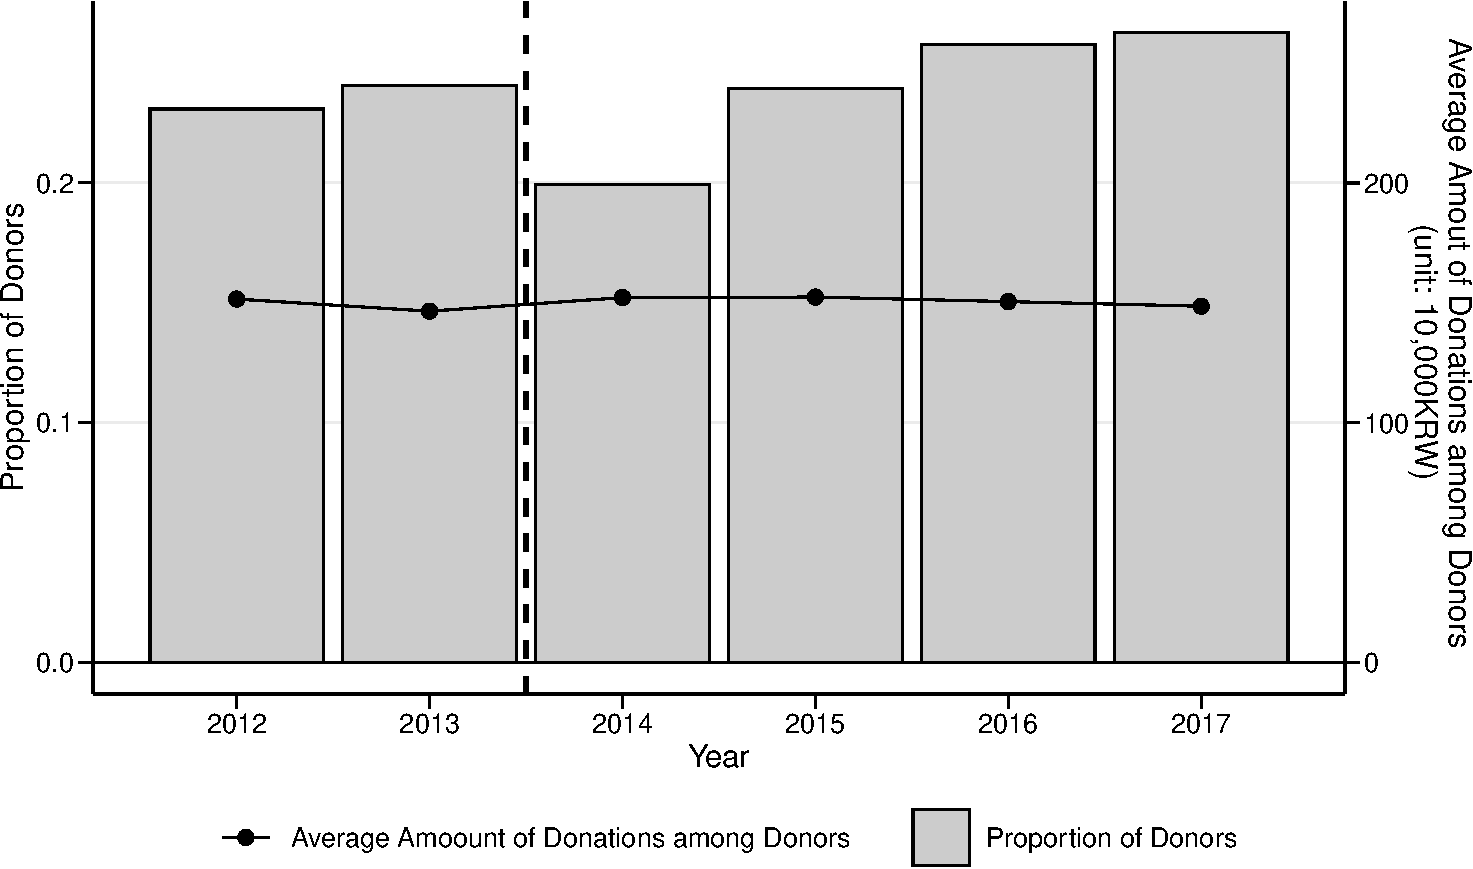
\includegraphics{C:/Users/katoo/Desktop/NASTAB/paper/draft_files/figure-latex/SummaryGiving-1} 

}

\caption{Proportion of Donors and Average Donations among Donors. Notes: The left and right axises measure prooortion of donors (grey bars) and the average amount of donations among donors (solid line), respectively.}\label{fig:SummaryGiving}
\end{figure}

各所得グループの寄付のトレンドを確認する前に、
全体的な寄付行動の傾向を図\ref{fig:SummaryGiving}に示した。
2012年から2017年にかけて、寄付者の割合は約24\%である。
税制改革直後の寄付者の割合は所得控除のもとでの寄付者の割合を下回ったが、
時間を通じて寄付者が増えている(グレーのバー)。
また、寄付者に限定した平均寄付額(黒の実線)は約1.5 million KRW(平均所得の約7\%)
で時間を通じて安定している。
寄付していない人も含めると、平均寄付額は358,600 KRW(平均所得の約2\%)である\footnote{欧米圏の寄付との簡単な比較があると文化差が伝わるかも(コメント)}。

\begin{figure}[t]

{\centering 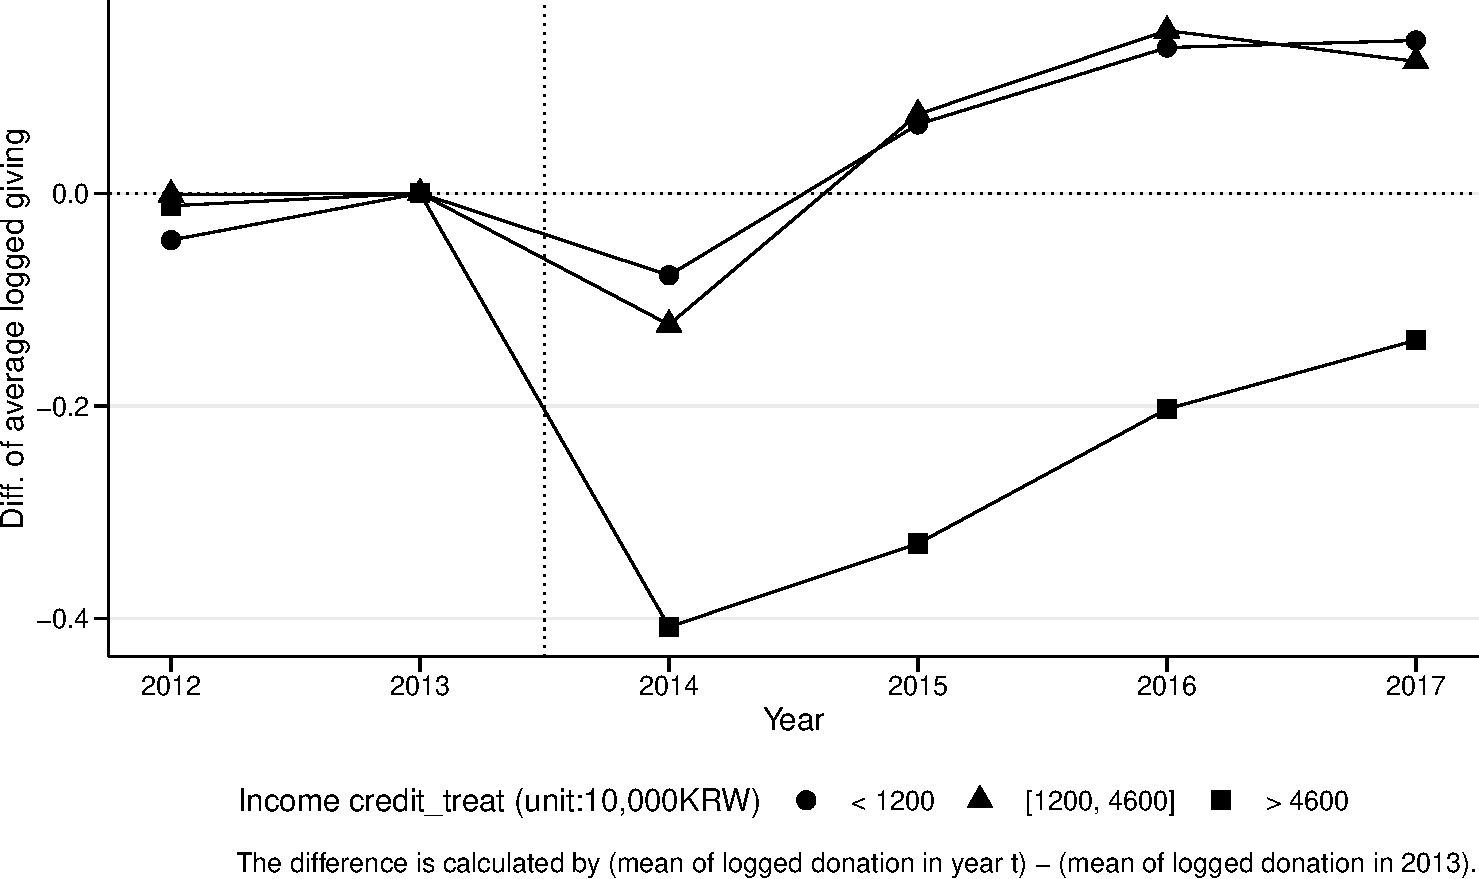
\includegraphics{C:/Users/katoo/Desktop/NASTAB/paper/draft_files/figure-latex/SummaryGivingOverall-1} 

}

\caption{Average Logged Giving by Three Income Groups. Notes: We created three income groups, with the relative price of giving rising (circle), unchanged (triangle), and falling (square) between 2013 and 2014. The group averages are normalized to be zero in 2013.}\label{fig:SummaryGivingOverall}
\end{figure}

図\ref{fig:SummaryGivingOverall}は
税インセンティブの変化に基づいた所得グループごとの平均寄付額を示している(非寄付者も含めている)。
この図から価格効果を観察できる。言い換えれば、税インセンティブは寄付行動を促進していることが観察される。
2015年以降、税制改革によって税インセンティブが拡大した(もしくは変化しなかった)人は所得控除時よりも増えているが、
税インセンティブが縮小した人は所得控除時よりも減少している。
また、寄付者に限定した平均寄付額と寄付者の割合のトレンドを所得グループごとに見ると、
似たような傾向が観察された
(補論\ref{addtab}の図\ref{fig:SummaryGivingIntensive}と図\ref{fig:SummaryGivingExtensive})。
ただし、寄付者に限定した平均寄付のトレンドを見ると、
図\ref{fig:SummaryGivingOverall}ほどはっきりとした価格効果を観察できない。

また、すべての所得グループの2014年の平均寄付額は2013年のそれを下回っている。
これはいくつかの可能性が考えられる。
第一に、税制改革のアナウンスメント効果である。
2014年の税制改革は2013年に告知されているので、
税インセンティブが縮小する所得グループにおいては、
2013年の寄付額を増やし、2014年の寄付額を減らすという異時点間の代替効果が予想される。
しかしながら、これは税インセンティブが拡大する所得グループの寄付額が減少した事実を説明できない。
第二の可能性は、制度の学習効果が考えられる。
税制改革直後は、税額控除によって自分が寄付によって節税しやすくなったかどうかが分からないので、
税インセンティブが拡大する所得グループでも寄付額は減少した。
それ以降、税インセンティブが拡大した納税者は自分が寄付によって節税しやすくなることを学習し、
寄付額を所得控除時よりも増やしたと考えられる。

寄付価格の変動は寄付控除の申告の有無でも生じる。
寄付控除を申告した場合の寄付の相対価格は図\ref{fig:SummaryPrice}に示した通りである一方で、
寄付控除を申告しない場合の寄付の相対価格は1である。
よって、控除の有無によって寄付の相対価格は変化する。
しかしながら、寄付控除の申告は自己選択なので、内生的である。
後に述べるように、この内生性を解決するために操作変数が必要である。

寄付控除の申告行動において、申告コストは大きな障害となっている可能性が高い。
補論\ref{addtab}の図\ref{fig:SummaryGivingIntensiveDist}に示しているように、
寄付控除の申告の有無によって、寄付者に限定した寄付額の分布は大きく変化しない。
これは寄付控除の申告の有無は、控除によって得られる便益の差よりも
申告するためのコストの差で説明できることを示唆している。

\begin{figure}[t]

{\centering 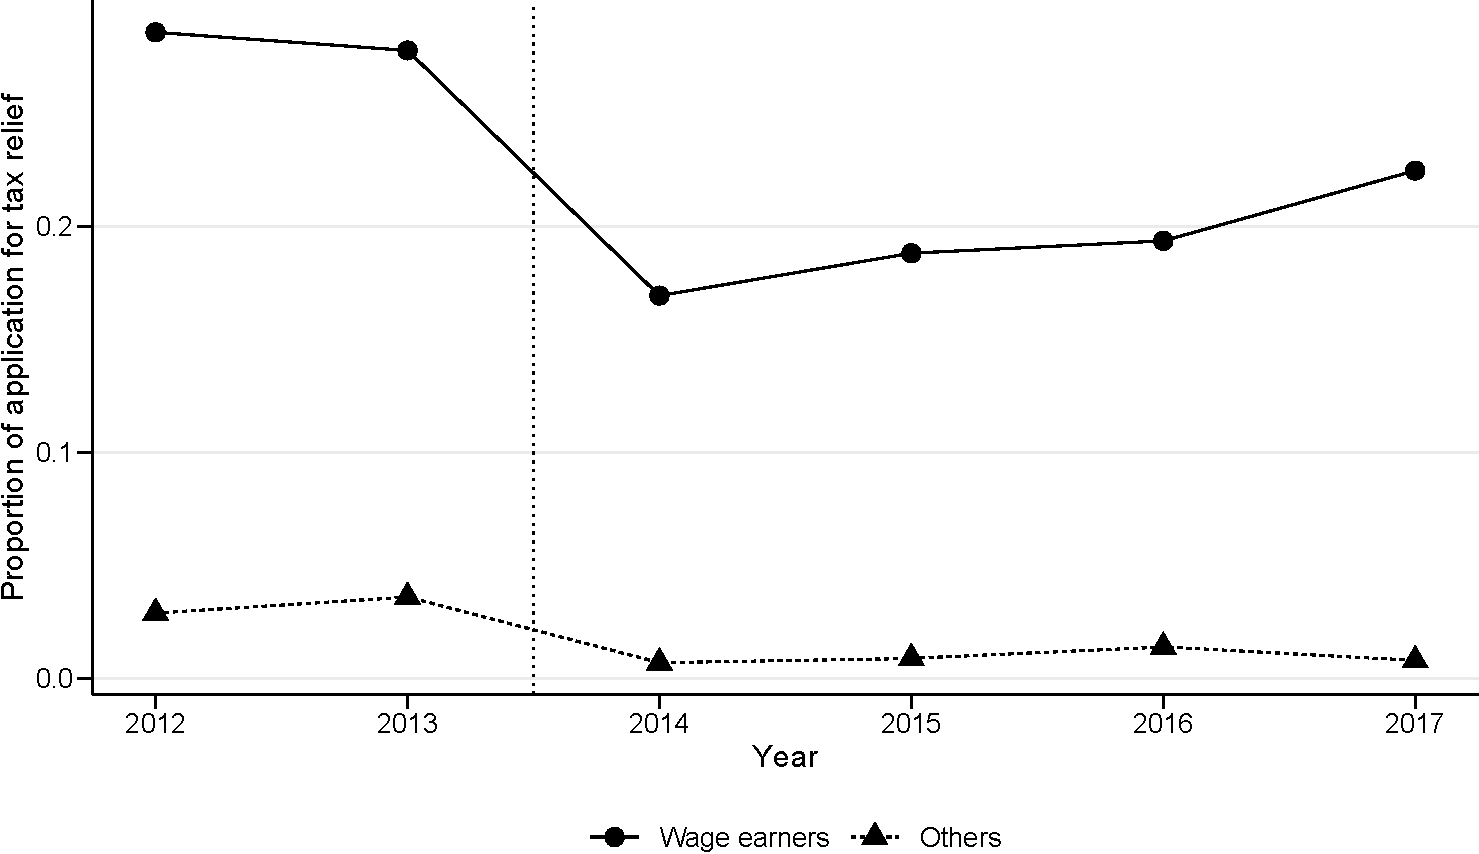
\includegraphics{C:/Users/katoo/Desktop/NASTAB/paper/draft_files/figure-latex/SummaryReliefbyEarner-1} 

}

\caption{Share of Tax Relief by Wage Earners. Notes: A solid line is the share of applying for tax relief among wage eaners. A dashed line is the share of applying for tax relief other than wage earners.}\label{fig:SummaryReliefbyEarner}
\end{figure}

以上を踏まえて、
我々は申告コストの要素の一つであるレコードキーピングに関する制度背景を第二の識別戦略として用いる。
先に述べたように、自営業者は寄付控除を申請するまで寄付の領収書(証明書)を保持しておく必要がある一方で、
給与所得者は会社を通じてその証明書をいつでも提出でき、
その後の申請も会社に手続きを依頼できる。
すなわち、給与所得者は自営業者よりも申告コストが低いことが予想される。
事実、図\ref{fig:SummaryReliefbyEarner}
給与所得者の控除の申請比率は自営業者よりもすべての期間を通じて高いことが分かる\footnote{寄付者に限定した控除の申告比率についても、給与所得者の方が自営業者よりも高い
  (補論\ref{addtab}の図\ref{fig:SummaryReliefbyEarner2})。}。
我々は給与所得者ダミーをレコードキーピングのコストの代理変数として操作変数に用いる。

\hypertarget{estimation}{%
\section{Empirical Strategy}\label{estimation}}

Almunia et al. (2020) に従い、我々は二種類の弾力性を推定する。
第一に、intensive-margin price elasiticityであり、
1\%の価格上昇で寄付者の寄付額が何\%増えるかを示している。
第二に、extensive-margin price elasiticityであり、
1\%の価格上昇で寄付者比率が何\%増えるかを示している。
第\ref{nastab}節で説明したように、
我々は2014年の税制改革による税インセンティブの変化を用いたDIDと
申告コストによる寄付控除の申請の有無を捉えた操作変数法の二つを組み合わせた識別戦略を用いる。

intensive-margin price elasticityは、
寄付者に限定して以下のtwo-way fixed effect modelを推定する。
\begin{align}
  \ln g_{it} = \theta_i + \gamma (R_{it} \times \ln (1 - s_{it}))
    + \beta X_{it} + \lambda_t + u_{it}, \label{eq:intensive}
\end{align}
ここで、\(X_{it}\)は課税前所得(\(y_{it}\))を含んだ共変量ベクトル、
\(\theta_i\)と\(\lambda_t\)はそれぞれ個人固定効果と時間固定効果である。
\(u_{it}\)はidiosyncratic errorである。
アウトカム変数\(\ln g_{it}\)は\(t\)年に寄付した人\(i\)の寄付額の対数値である。
寄付価格は\(R_{it} \times \ln (1 - s_{it})\)であり、
ここで、\(R_{it}\)は控除申請のダミー変数、\(s_{it}\)は税インセンティブである\footnote{寄付価格は\(\ln(1 - R_{it}s_{it})\)とも書ける。
  これは\(R_{it} \times \ln (1 - s_{it})\)と一致する。
  なぜなら、\(R_{it} = 0\)のとき、\(\ln(1) = 0\)となり、
  \(R_{it} = 1\)のとき、\(\ln(1 - s_{it})\)となる。}。
したがって、関心のあるパラメータは\(\gamma\)であり、
これがintensive-margin price elasticityを示す。

extensive-margin price elasticityの推定式は
two-way fixed effect付きの線形確率モデルである。
すなわち、
\begin{align}
  D_{it} = \theta_i + \delta (R_{it} \times \ln (1 - s_{it}))
    + \beta X_{it} + \lambda_t + \eta_{it}, \label{eq:extensive}
\end{align}
である。
アウトカム変数\(D_{it}\)は正の寄付額が観測されたら1を取るダミー変数である:\(D_{it} = 1[g_{it} > 0]\)。
ここで関心のあるパラメータは\(\delta\)である。
アウトカム変数は二値なので、このパラメータを弾力性として直接解釈できない。
extensive-margin price elasticityは\(\hat{\delta} / \bar{D}\)で得られる
(\(\bar{D}\)は\(D_{it}\)の標本平均)。

この推定式における二つの内生性に対する対処法について議論する。
第一に、
2014年の税制改革による税インセンティブの変化を寄付価格の外生的な変動要因として用いるが、
寄付価格の内生性は完全に排除できない。
寄付控除を申請した場合の寄付価格を以下のようになる。
\begin{align}
  1 - s_{it} =
  \begin{cases}
    1 - T'_t(y_{it} - g_{it})  \quad\text{if}\quad t < 2014  \\
    1 - m \quad\text{if}\quad t \ge 2014
  \end{cases},
\end{align}
ここで、\(T'_t(\cdot)\)は\(t\)年の限界所得税率、\(m\)は税額控除率(\(m = 0.15\))である。
寄付価格は2014年の税制改革だけではなく、
所得控除が適用される期間において、寄付額(\(g_{it}\))にも依存する。
これは\emph{last}-unit priceと呼ばれるものであり、この寄付価格は寄付額について内生的である\footnote{寄付額によるインセンティブの操作について、次の二つの可能性が考えられる。
  第一に、納税者は寄付額を減らすことで、所得税率を高められる(寄付価格を高められる)。
  第二に、納税者は寄付額を増やすことで、所得税率を下げられる(節税の額を増やせる)。}。

本研究は、過去の研究にならい、
last-unit priceの代わり(もしくはその操作変数)として\emph{first}-unit priceを用いる。
last-unit priceは最終的な寄付額で寄付価格を計算する一方で、
first-unit priceは寄付額をゼロとして寄付価格を計算する\footnote{first-unit priceは
  最初の1単位を寄付するかどうかの意思決定時に直面する価格として解釈できる。}。
すなわち、
\begin{align}
  1 - s^f_{it} =
  \begin{cases}
    1 - T'_t(y_{it} - 0)  \quad\text{if}\quad t < 2014  \\
    1 - m \quad\text{if}\quad t \ge 2014
  \end{cases}.
\end{align}
ただし、税額控除が適用される期間においては、
寄付価格が寄付額に依存しないので、last-unit priceとfirst-unit priceは一致する。

第二に、寄付控除申告の自己選択による内生性である。
申告コストがないとき、節税による便益を得られるので、
寄付者は全員寄付控除を申請するべきである。
しかしながら、我々のデータでは、寄付者の割合は24\%であるにも関わらず、
控除を申告した人の割合は10\%である(表\ref{tab:SummaryCovariate})。
また、補論\ref{addtab}の図\ref{fig:SummaryGivingIntensiveDist}に示しているように、
寄付控除の申告の有無によって、寄付者に限定した寄付額の分布は大きく変化しない。
これは寄付控除の申告行動において、申告コストは大きな障害となっている可能性が高いことを示唆している。

本研究はレコードキーピングの制度が給与所得者と自営業者で異なることを利用して、
給与所得者ダミー(\(WE_{it}\))をレコードキーピングのコストの代理変数として操作変数に用いる\footnote{給与所得者ダミーを操作変数として用いるためには、
  共変量で条件づけたとき、この変数が\(u_{it}\)と\(\eta_{it}\)と独立していることを仮定する必要がある。
  ただし、給与所得者ダミーと固定効果の相関は許容できる。
  我々は、所得や業種をコントロールすれば、
  給与所得者であるかどうかは寄付行動に直接的な影響を持たないと考えている。}。
自営業者は寄付控除を申請するまで寄付の領収書(証明書)を保持しておく必要がある一方で、
給与所得者は会社を通じてその証明書をいつでも提出できるので、
給与所得者は自営業者よりも申告コストが低いことが予想される。

Wooldridge (2010) に従い、
我々は給与所得者ダミーを操作変数とした三つのアプローチを用いる\footnote{以降ではintensive-margin price elasticityの推定式を用いて説明するが、
  extensive-margin price elasticityの推定についても同じ方法が適用できる。}。
第一に、給与所得者ダミーとfirst-unit priceの交差項を
\(R_{it} \times \ln (1 - s^f_{it})\)の操作変数として用いる。
すなわち、intensive-margin price elasiticityの推定式は
\begin{align}
  \ln g_{it} = \theta_i + \gamma (R_{it} \times \ln (1 - s^f_{it}))
    + \beta X_{it} + \lambda_t + u_{it}, \label{eq:intensive2}
\end{align}
であり、
\(R_{it} \times \ln (1 - s^f_{it})\)の操作変数を\(WE_{it} \times \ln(1 - s^f_{it})\)とする\footnote{last-unit priceを用いて弾力性を推定する場合、
  \eqref{eq:intensive}もしくは\eqref{eq:extensive}の説明変数
  \(R_{it} \times \ln (1 - s_{it})\)の操作変数として
  \(WE_{it} \times \ln(1 - s^f_{it})\)を用いる。}。

残りの二つのアプローチは寄付申告の傾向スコアを用いるものである。
傾向スコアは以下のモデルをプロビット推定した予測確率で得られる。
\begin{align}
  R_{it} = 1[
    \alpha_0 + \alpha_1 WE_{it} + \alpha_2 \ln(1 - s^f_{it})
    + \alpha_3 X_{it} + u_{it0} > 0
  ] \label{eq:selection}
\end{align}

我々は全期間のサンプルを用いた推定(pooled model)と
年で分割したサブサンプルを用いた推定(separeted model)で傾向スコア\(\hat{P}_{it}\)を得た。
前者のモデルは式\eqref{eq:selection}の係数が時間に対して一定であると仮定している一方で、
後者のモデルは推定される係数が時間に依存することを許容したモデルである。

傾向スコアを用いた第二のアプローチは
式\eqref{eq:intensive2}の説明変数\(R_{it} \times \ln (1 - s^f_{it})\)の操作変数として
\(\hat{P}_{it} \times \ln (1 - s^f_{it})\)を用いる。
第三のアプローチは式\eqref{eq:intensive2}の説明変数\(R_{it} \times \ln (1 - s^f_{it})\)
の代わりに\(\hat{P}_{it} \times \ln (1 - s^f_{it})\)を用いる。すなわち、
我々は以下のモデルを推定する。
\begin{align}
  \ln g_{it} = \theta_i + \gamma (\hat{P}_{it} \times \ln (1 - s^f_{it}))
    + \beta X_{it} + \lambda_t + u_{it}, \label{eq:intensive3}
\end{align}

\hypertarget{result}{%
\section{Estimation Results}\label{result}}

\hypertarget{main-results}{%
\subsection{Main Results}\label{main-results}}

\begin{table}

\caption{\label{tab:MainIntensive}Intensive-Margin Tax-Price Elasticity}
\centering
\fontsize{8}{10}\selectfont
\begin{threeparttable}
\begin{tabular}[t]{lcccccc}
\toprule
\multicolumn{1}{c}{ } & \multicolumn{3}{c}{FE} & \multicolumn{3}{c}{FE-2SLS} \\
\cmidrule(l{3pt}r{3pt}){2-4} \cmidrule(l{3pt}r{3pt}){5-7}
  & (1) & (2) & (3) & (4) & (5) & (6)\\
\midrule
Applying tax relief x log(first price) & \num{-0.748}*** &  &  & \num{-1.400}*** & \num{-1.437}*** & \num{-1.540}***\\
 & (\num{0.225}) &  &  & (\num{0.411}) & (\num{0.363}) & (\num{0.375})\\
PS of applying tax relief x log(first price) &  & \num{-1.544}*** & \num{-1.515}*** &  &  & \\
 &  & (\num{0.388}) & (\num{0.367}) &  &  & \\
log(income) & \num{1.408} & \num{0.833} & \num{0.824} & \num{0.937} & \num{0.909} & \num{0.830}\\
 & (\num{1.113}) & (\num{1.121}) & (\num{1.121}) & (\num{1.119}) & (\num{1.098}) & (\num{1.094})\\
\midrule
First-stage: Instrument &  &  &  & 0.638 & 1.075 & 0.984\\
 &  &  &  & [468.1] & [534.6] & [662.2]\\
Num.Obs. & \num{7004} & \num{6975} & \num{6975} & \num{6975} & \num{6975} & \num{6975}\\
FE: year & X & X & X & X & X & X\\
FE: pid & X & X & X & X & X & X\\
FE: indust & X & X & X & X & X & X\\
FE: area & X & X & X & X & X & X\\
Square of age & X & X & X & X & X & X\\
Instrument &  &  &  & WE x Price & PS x Price & PS x Price\\
Method of PS &  & Pool & Separate &  & Pool & Separate\\
\bottomrule
\multicolumn{7}{l}{\rule{0pt}{1em}* p $<$ 0.1, ** p $<$ 0.05, *** p $<$ 0.01}\\
\end{tabular}
\begin{tablenotes}
\item Notes: $^{*}$ $p < 0.1$, $^{**}$ $p < 0.05$, $^{***}$ $p < 0.01$. Standard errors are clustered at individual level. A square bracket is wald statistics of instrument.
\end{tablenotes}
\end{threeparttable}
\end{table}

表\ref{tab:MainIntensive}は寄付者に限定した
寄付の価格弾力性(intensive-margin price elasticity)の推定結果である。
モデル(1)は標準的なtwo-way fixed effect modelであり、
操作変数による寄付控除の自己選択を制御していない。
このモデルはintensive-margin price elasticityが-0.748であることを示している。
言い換えれば、税インセンティブによる寄付価格が1\%上昇することによって、
寄付者に限定した寄付額が約0.75\%減少する。
モデル(2)-(6)は操作変数法による寄付控除の自己選択を制御したときの
intensive-margin price elasticityを示している。
その結果、推定方法に関わらず、intensive-margin price elasticityは約-1.5になった。
言い換えれば、寄付控除の自己選択を制御したとき、
1\%の寄付価格の上昇によって、寄付者に限定した寄付額が1.5\%減少する。
したがって、操作変数法による寄付控除の自己選択を制御したとき、
intensive-margin price elasticityはより弾力的に推定された\footnote{モデル(4)-(6)に示した個人固定効果と時間固定効果を含めた二段階最小二乗法(FE-2SLS)を用いて、
  我々は操作変数の弱相関の程度を確認できる。その結果、操作変数の種類に関わらず、F値は450以上ある。
  したがって、操作変数法によってintensive-margin price elasticityがより弾力的になった結果は
  操作変数の弱相関によるものではない。}。

\begin{table}

\caption{\label{tab:MainExtensive}Extensive-Margin Tax-Price Elasticity}
\centering
\fontsize{8}{10}\selectfont
\begin{threeparttable}
\begin{tabular}[t]{lcccccc}
\toprule
\multicolumn{1}{c}{ } & \multicolumn{3}{c}{FE} & \multicolumn{3}{c}{FE-2SLS} \\
\cmidrule(l{3pt}r{3pt}){2-4} \cmidrule(l{3pt}r{3pt}){5-7}
  & (1) & (2) & (3) & (4) & (5) & (6)\\
\midrule
Applying tax relief x log(first price) & \num{-2.800}*** &  &  & \num{-0.464}*** & \num{-0.563}*** & \num{-0.738}***\\
 & (\num{0.074}) &  &  & (\num{0.176}) & (\num{0.120}) & (\num{0.116})\\
PS of applying tax relief x log(first price) &  & \num{-0.452}*** & \num{-0.566}*** &  &  & \\
 &  & (\num{0.107}) & (\num{0.101}) &  &  & \\
log(income) & \num{0.975}*** & \num{1.950}*** & \num{1.844}*** & \num{2.121}*** & \num{2.072}*** & \num{1.986}***\\
 & (\num{0.233}) & (\num{0.279}) & (\num{0.278}) & (\num{0.279}) & (\num{0.261}) & (\num{0.256})\\
\midrule
Implied price elasticity & -10.799*** & -1.741*** & -2.181*** & -1.788*** & -2.169*** & -2.841***\\
 & (0.287) & (0.411) & (0.388) & (0.678) & (0.463) & (0.448)\\
First-stage: Instrument &  &  &  & 0.289 & 0.803 & 0.768\\
 &  &  &  & [276.6] & [311.7] & [361.9]\\
Num.Obs. & \num{27017} & \num{26863} & \num{26863} & \num{26863} & \num{26863} & \num{26863}\\
FE: year & X & X & X & X & X & X\\
FE: pid & X & X & X & X & X & X\\
FE: indust & X & X & X & X & X & X\\
FE: area & X & X & X & X & X & X\\
Square of age & X & X & X & X & X & X\\
Instrument &  &  &  & WE x Price & PS x Price & PS x Price\\
Method of PS &  & Pool & Separate &  & Pool & Separate\\
\bottomrule
\multicolumn{7}{l}{\rule{0pt}{1em}* p $<$ 0.1, ** p $<$ 0.05, *** p $<$ 0.01}\\
\end{tabular}
\begin{tablenotes}
\item Notes: $^{*}$ $p < 0.1$, $^{**}$ $p < 0.05$, $^{***}$ $p < 0.01$. Standard errors are clustered at individual level. A square bracket is wald statistics of instrument.
\end{tablenotes}
\end{threeparttable}
\end{table}

表\ref{tab:MainExtensive}は寄付行動の有無の価格弾力性
(extensive-margin price elasticity)を示している。
モデル(1)は標準的なtwo-way fixed effect modelである。
このモデルの寄付価格の係数は-2.8である。
しかしながら、先述の通り、
線型確率モデルなので、この係数を直接弾力性として解釈できない。
弾力性を得るために、この係数を寄付者の比率で割る必要がある。
その結果、操作変数による寄付控除の自己選択を制御しない場合、
extensive-margin price elasticityは約-10.8となった。
言い換えれば、1\%の価格上昇が寄付する確率を約10\%減少させる。

表\ref{tab:MainIntensive}と同様に、
表\ref{tab:MainExtensive}のモデル(2)-(6)は操作変数法によって寄付控除の自己選択を制御したモデルである。
その結果、推定方法に関わらず、寄付価格の係数は-0.738から-0.452の間に入っている。
これを価格弾力性に変換すると、-1.7から-2.8のレンジで得られた。
言い換えれば、寄付価格1\%の上昇によって、寄付をする確率が約1.7-2.8\%減少する。
したがって、操作変数によって寄付控除の自己選択を制御した場合、
extensive-margin price elasticityはより非弾力的に推定された。

\hypertarget{robustness-check}{%
\subsection{Robustness Check}\label{robustness-check}}

結果を解釈する前に、ここまでの推定結果が頑健に観察されることを確認する。

\noindent
\emph{Exclude Annoucement Effect}.
第\ref{nastab}節の図\ref{fig:SummaryGivingOverall}で示したように、
2014年の税制改革による税インセンティブの変化に関わらず、寄付額が減少している。
この一つの可能性として、税制改革が事前告知されたことによる異時点間の代替性が生じているかもしれない。
これを排除して弾力性を推定するために、
我々は事前のアナウンスメントによる異時点間の代替性が2013年と2014年のみで生じていることを仮定して、
2013年と2014年のデータを除いて弾力性を推定した。
推定結果を補論\ref{addtab}の
表\ref{tab:WoAnnoucementIntensive}と\ref{tab:WoAnnouncementExtensive}に示した。
その結果、推定値は大きく変化しなかった。
また、操作変数による寄付控除の自己選択の制御によって、
intensive-margin price elasticityがより弾力的に推定されるとともに、
extensive-margin price elasticityが非弾力的に推定されることも観察された。

\noindent
\emph{Last-unit price elasticity}.
First-unit priceは寄付していないときに直面する寄付価格である。
意思決定者が直面する価格はfirst-unit priceではなく、last-unit priceである。
Last-unit priceは意思決定者の寄付額を用いて計算した寄付価格である。
Last-unit priceを用いて、
我々は価格弾力性の推定し、その結果を補論\ref{addtab}の
表\ref{tab:LastIntensive}と\ref{tab:LastExtensive}に示した。
Last-unit priceは寄付額に対して内生的であるので、
我々は表\ref{tab:MainIntensive}と同じ操作変数法でこれに対応した。
その結果、first-unit priceを用いた価格弾力性と比べて、
intensive-margin price elasticityと
extensive-margin price elasticityはより弾力的に推定された。
とくに、extensive-margin price elasticityは2倍近く弾力的になった。
また、操作変数による寄付控除の自己選択の制御によって、
intensive-margin price elasticityがより弾力的に推定されるとともに、
extensive-margin price elasticityが非弾力的に推定されることも観察された。

\noindent
\emph{Conventional Estimation Strategy.}
これまでの弾力性を推定した研究がLast-unit priceを用いた弾力性を推定するとき、
単にfirst-unit priceを操作変数として用いている。
過去の研究結果との比較をするために、
我々もこの方法にしたがってLast-unit priceを用いた弾力性を推定した。
推定結果を補論\ref{addtab}の表\ref{tab:MainElasticity}に示した。
その結果、Intensive-margin price elasticityは-1.9と推定されたのに対し、
extensive-margin price elasticityは-6.2と推定された\footnote{2014年の税制改革のアナウンスメント効果を排除するために、
  2013年と2014年のデータを除いた分析もした。
  推定結果は補論\ref{addtab}の表\ref{tab:WoAnnoucementElasticity}に示した。
  その結果、どちらの価格弾力性もより弾力的に推定された。
  この傾向はこれまでの結果と整合的である。}。
これは我々の方法で推定した結果
(補論\ref{addtab}の表\ref{tab:LastIntensive}と\ref{tab:LastExtensive})
よりも弾力的になった。

\noindent
\emph{Use those who applied for tax relief}.
弾力性を推定した過去の研究は寄付控除を申告した人に限定したデータを用いている。
こうした研究の結果と比較するために、我々も寄付控除を申告した人に限定した分析を行った。
寄付控除を申告している人は必ず寄付をしているので、
我々はintensive-margin price elasticityのみを推定できる。
推定結果を補論\ref{addtab}の表\ref{tab:R1Elasticity}に示した。
その結果、first-unit priceを用いたとき、
intensive-margin price elasticityは約-1.2となった。
また、last-unit priceを用いたとき、
価格弾力性は約-1.3となった\footnote{価格のダイナミックな効果を捉えるために、
  寄付価格と所得のリード変数とラグ変数を加えると、価格弾力性は統計的に非有意となった。
  また、我々は所得に対する寄付価格の内生性を考慮した\(k\)-th difference modelも推定し、
  その結果を補論\ref{addtab}の表\ref{tab:KdiffElasticity}に示した。
  このモデルの推定結果はintensive-margin price elasticityの絶対値は最大でも5となった。}。
これは控除を申請していない人を含めた分析(表\ref{tab:MainIntensive})の
弾力性と非常に近い値となっている。

\hypertarget{interpretation}{%
\subsection{Interpretation}\label{interpretation}}

サンプルを3つのタイプに分割する。

\begin{enumerate}
\def\labelenumi{\arabic{enumi}.}
\tightlist
\item
  Always declarer:給与所得者かどうかによる申告コストの水準に関わらず、寄付控除を申告する人
\end{enumerate}

\begin{itemize}
\tightlist
\item
  2014年の税制改革によって価格のwitin-variationは存在するが、常に寄付をする
\item
  したがって、このグループのextensive-marginの価格弾力性は(絶対値の意味で)0
\end{itemize}

\begin{enumerate}
\def\labelenumi{\arabic{enumi}.}
\tightlist
\item
  Start declarer:申告コストの水準が自営業者から給与所得者の水準まで下がることで、寄付控除を申告する人
\item
  Never declarer:給与所得者かどうかによる申告コストの水準に関わらず、寄付控除を申告しない人
\end{enumerate}

\begin{itemize}
\tightlist
\item
  常に価格が1であるにも関わらず、寄付額や寄付の意思決定が変化する
\item
  intensive-margin・extensive-marginの価格弾力性は無限大に発散する
\end{itemize}

したがって、3タイプの価格弾力性の大きさは絶対値の意味で以下のような関係になっているのではないだろうか?

\begin{itemize}
\tightlist
\item
  Intensive-margin:Always \textless{} Start \textless{} Never

  \begin{itemize}
  \tightlist
  \item
    ただし、これは後藤さんのロジックである「申告で常に得するような人は多少の価格変動に動じない」を借りている
  \end{itemize}
\item
  Extensive-margin:Always \textless{} Start \textless{} Never
\end{itemize}

Intensive-marginのFEはAlwaysとStartに過重を置いて推定している(というか、Neverタイプが多くない)。
Extensive-marginのFEはNeverに過重を置いて推定している。
しかしながら、FE-2SLSはStartの弾力性を捉えているはずなので、

\begin{itemize}
\tightlist
\item
  Intensive-margin:FE \textless{} FE-2SLS
\item
  Extensive-margin:FE-2SLS \textless{} FE
\end{itemize}

となった。

\newpage

\hypertarget{appendix-appendix}{%
\appendix}


\hypertarget{addtab}{%
\section{Additional Tables and Figures}\label{addtab}}

\begin{figure}[H]

{\centering 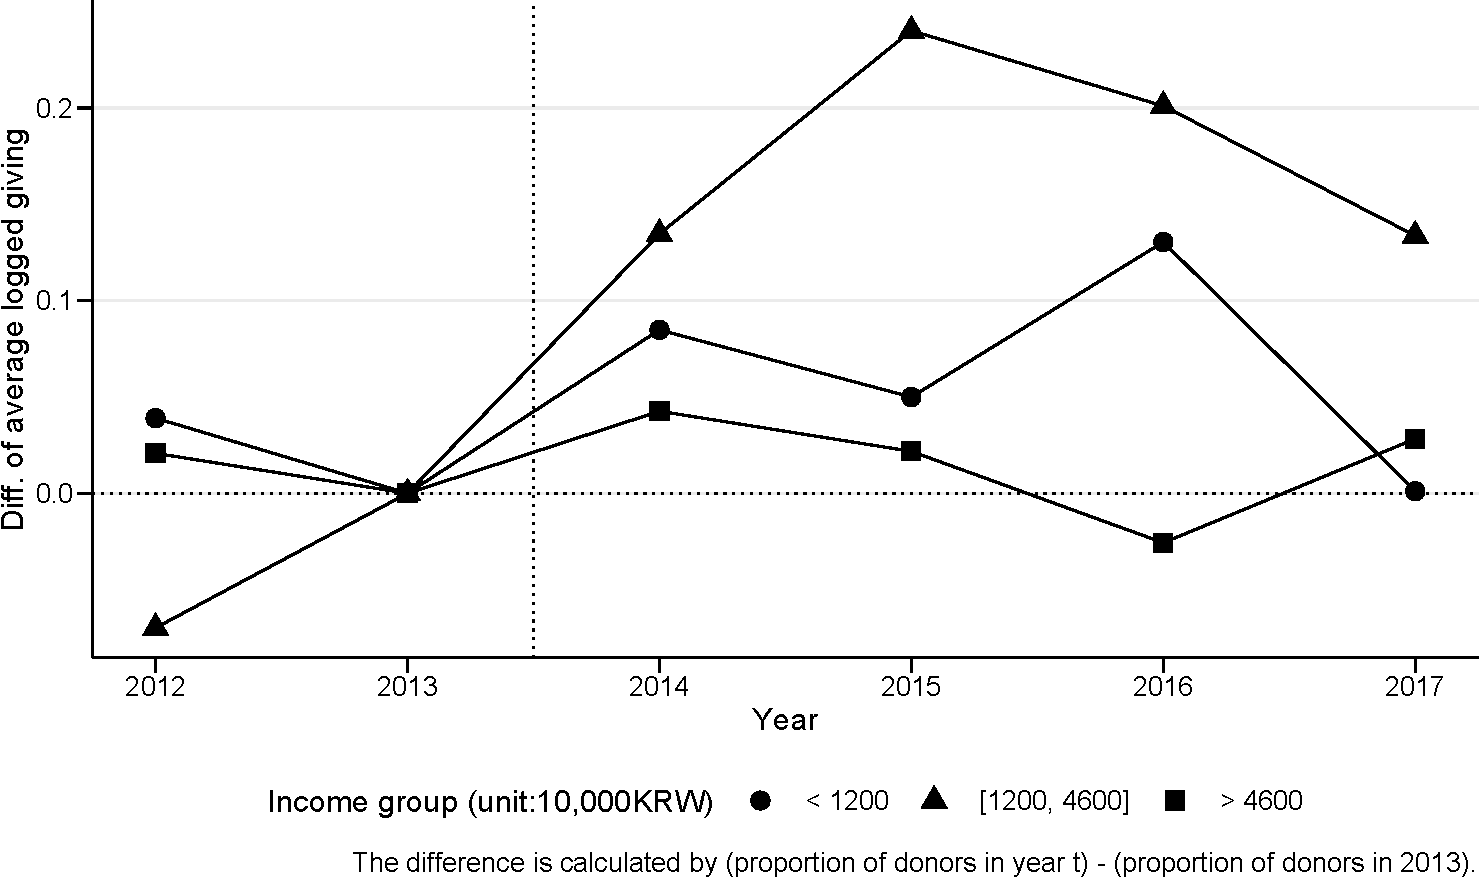
\includegraphics{C:/Users/katoo/Desktop/NASTAB/paper/draft_files/figure-latex/SummaryGivingIntensive-1} 

}

\caption{Average Logged Giving by Three Income Groups Conditional on Donors. Notes: We created three income groups, with the relative price of giving rising (circle), unchanged (triangle), and falling (square) between 2013 and 2014. The group averages are normalized to be zero in 2013.}\label{fig:SummaryGivingIntensive}
\end{figure}

\begin{figure}[H]

{\centering 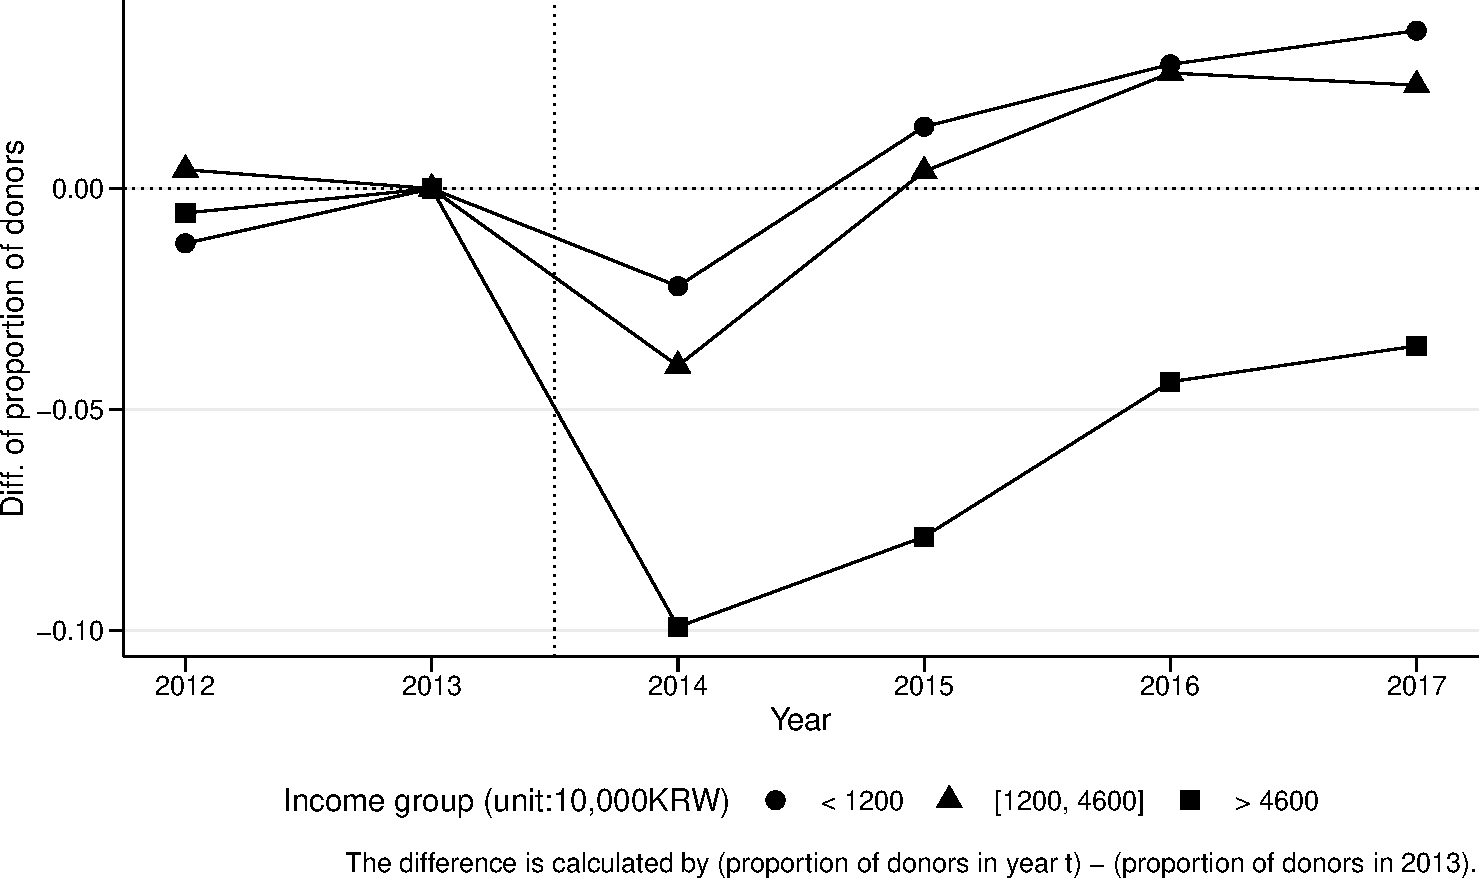
\includegraphics{C:/Users/katoo/Desktop/NASTAB/paper/draft_files/figure-latex/SummaryGivingExtensive-1} 

}

\caption{Proportion of Donors by Three Income Groups. Notes: We created three income groups, with the relative price of giving rising (circle), unchanged (triangle), and falling (square) between 2013 and 2014. The group averages are normalized to be zero in 2013.}\label{fig:SummaryGivingExtensive}
\end{figure}

\begin{figure}[H]

{\centering 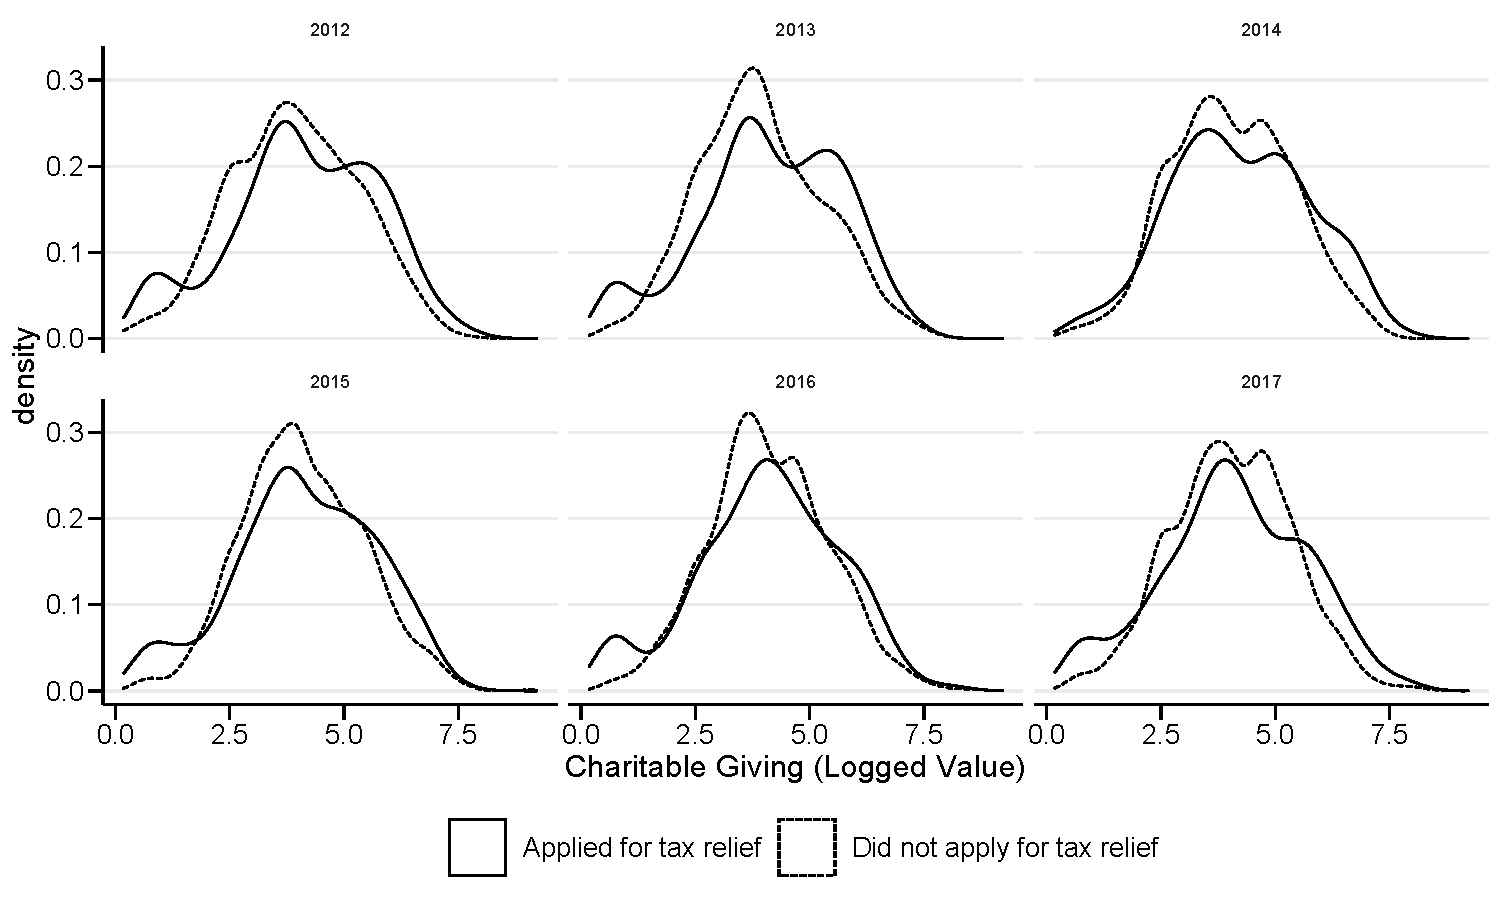
\includegraphics{C:/Users/katoo/Desktop/NASTAB/paper/draft_files/figure-latex/SummaryGivingIntensiveDist-1} 

}

\caption{Estimated Distribution of Charitable Giving among Donors in Each Year}\label{fig:SummaryGivingIntensiveDist}
\end{figure}

\begin{figure}[H]

{\centering 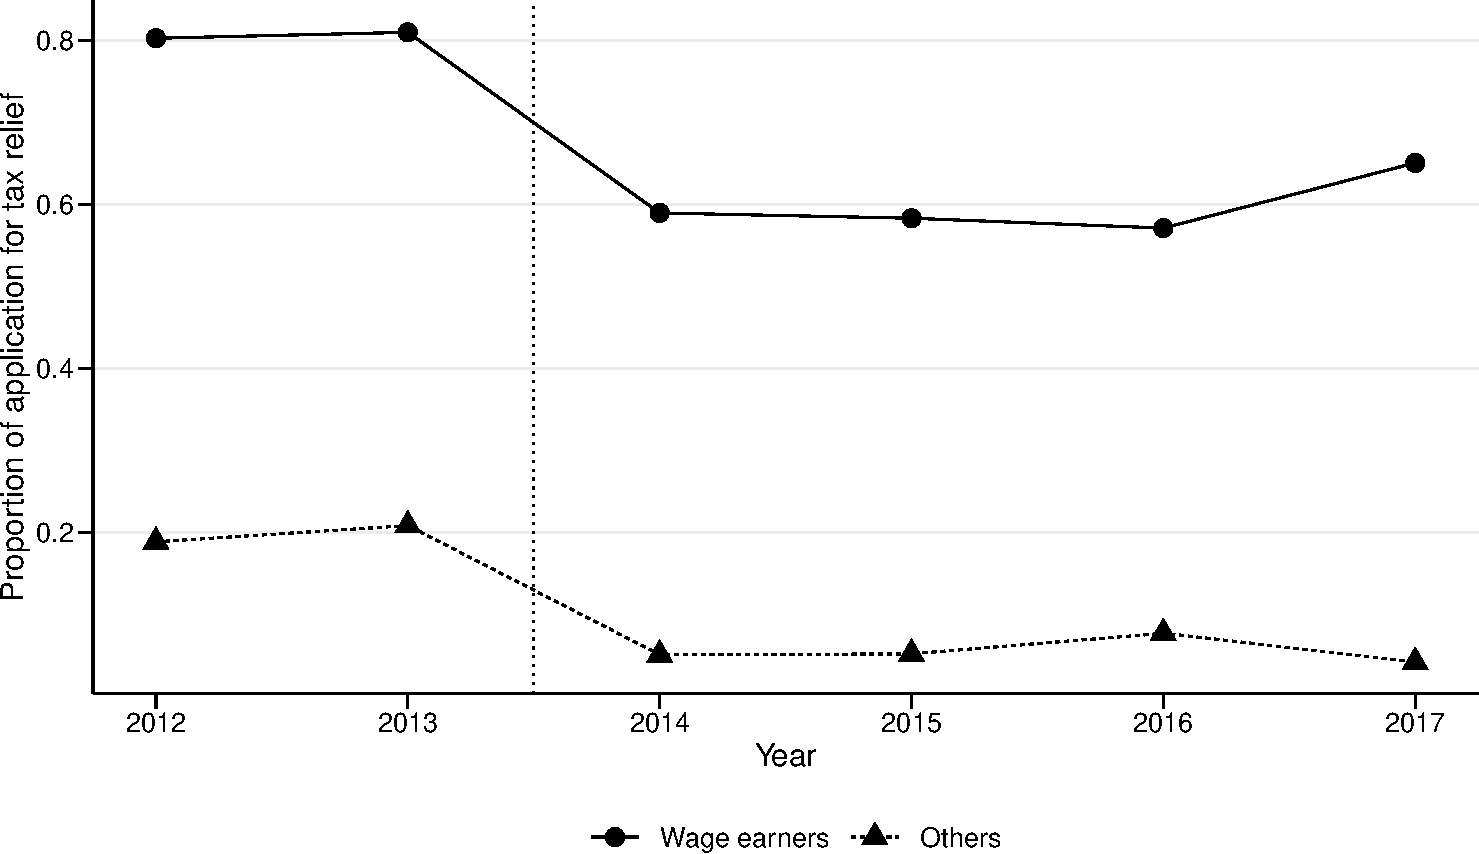
\includegraphics{C:/Users/katoo/Desktop/NASTAB/paper/draft_files/figure-latex/SummaryReliefbyEarner2-1} 

}

\caption{Share of Tax Relief by Wage Earners Conditional on Donors. Notes: A solid line is the share of applying for tax relief among wage eaners. A dashed line is the share of applying for tax relief other than wage earners.}\label{fig:SummaryReliefbyEarner2}
\end{figure}

\begin{table}[!h]

\caption{\label{tab:WoAnnoucementIntensive}Intensive-Margin Tax-Price Elasticity Excluding 2013 and 2014 data}
\centering
\fontsize{8}{10}\selectfont
\begin{threeparttable}
\begin{tabular}[t]{lcccccc}
\toprule
\multicolumn{1}{c}{ } & \multicolumn{3}{c}{FE} & \multicolumn{3}{c}{FE-2SLS} \\
\cmidrule(l{3pt}r{3pt}){2-4} \cmidrule(l{3pt}r{3pt}){5-7}
  & (1) & (2) & (3) & (4) & (5) & (6)\\
\midrule
Applying tax relief x log(first price) & \num{-0.765}** &  &  & \num{-1.560}** & \num{-1.505}*** & \num{-1.548}***\\
 & (\num{0.351}) &  &  & (\num{0.609}) & (\num{0.479}) & (\num{0.490})\\
PS of applying tax relief x log(first price) &  & \num{-1.783}*** & \num{-1.715}*** &  &  & \\
 &  & (\num{0.569}) & (\num{0.542}) &  &  & \\
log(income) & \num{0.041} & \num{-0.990} & \num{-0.955} & \num{-0.567} & \num{-0.541} & \num{-0.561}\\
 & (\num{1.460}) & (\num{1.477}) & (\num{1.467}) & (\num{1.440}) & (\num{1.427}) & (\num{1.418})\\
\midrule
First-stage: Instrument &  &  &  & 0.638 & 1.075 & 0.984\\
 &  &  &  & [468.1] & [534.6] & [662.2]\\
Num.Obs. & \num{4863} & \num{4844} & \num{4844} & \num{4844} & \num{4844} & \num{4844}\\
Square of age & X & X & X & X & X & X\\
Instrument &  &  &  & WE x Price & PS x Price & PS x Price\\
Method of PS &  & Pool & Separate &  & Pool & Separate\\
\bottomrule
\multicolumn{7}{l}{\rule{0pt}{1em}* p $<$ 0.1, ** p $<$ 0.05, *** p $<$ 0.01}\\
\end{tabular}
\begin{tablenotes}
\item Notes: $^{*}$ $p < 0.1$, $^{**}$ $p < 0.05$, $^{***}$ $p < 0.01$. Standard errors are clustered at individual level. A square bracket is wald statistics of instrument.
\end{tablenotes}
\end{threeparttable}
\end{table}

\begin{table}[!h]

\caption{\label{tab:WoAnnouncementExtensive}Extensive-Margin Tax-Price Elasticity Excluding 2013 and 2014 data}
\centering
\fontsize{8}{10}\selectfont
\begin{threeparttable}
\begin{tabular}[t]{lcccccc}
\toprule
\multicolumn{1}{c}{ } & \multicolumn{3}{c}{FE} & \multicolumn{3}{c}{FE-2SLS} \\
\cmidrule(l{3pt}r{3pt}){2-4} \cmidrule(l{3pt}r{3pt}){5-7}
  & (1) & (2) & (3) & (4) & (5) & (6)\\
\midrule
Applying tax relief x log(first price) & \num{-2.970}*** &  &  & \num{-0.247} & \num{-0.607}*** & \num{-0.744}***\\
 & (\num{0.093}) &  &  & (\num{0.261}) & (\num{0.166}) & (\num{0.161})\\
PS of applying tax relief x log(first price) &  & \num{-0.503}*** & \num{-0.594}*** &  &  & \\
 &  & (\num{0.155}) & (\num{0.148}) &  &  & \\
log(income) & \num{1.134}*** & \num{1.919}*** & \num{1.837}*** & \num{2.260}*** & \num{2.110}*** & \num{2.054}***\\
 & (\num{0.278}) & (\num{0.328}) & (\num{0.327}) & (\num{0.320}) & (\num{0.293}) & (\num{0.290})\\
\midrule
Implied price elasticity & -11.121*** & -1.879*** & -2.221*** & -0.924 & -2.271*** & -2.782***\\
 & (0.347) & (0.580) & (0.553) & (0.974) & (0.622) & (0.604)\\
First-stage: Instrument &  &  &  & 0.276 & 0.828 & 0.798\\
 &  &  &  & [156.2] & [181.1] & [202.3]\\
Num.Obs. & \num{18207} & \num{18112} & \num{18112} & \num{18112} & \num{18112} & \num{18112}\\
Square of age & X & X & X & X & X & X\\
Instrument &  &  &  & WE x Price & PS x Price & PS x Price\\
Method of PS &  & Pool & Separate &  & Pool & Separate\\
\bottomrule
\multicolumn{7}{l}{\rule{0pt}{1em}* p $<$ 0.1, ** p $<$ 0.05, *** p $<$ 0.01}\\
\end{tabular}
\begin{tablenotes}
\item Notes: $^{*}$ $p < 0.1$, $^{**}$ $p < 0.05$, $^{***}$ $p < 0.01$. Standard errors are clustered at individual level. A square bracket is wald statistics of instrument.
\end{tablenotes}
\end{threeparttable}
\end{table}

\begin{table}[!h]

\caption{\label{tab:LastIntensive}Intensive-Margin Tax-Price Elasticity (Last-Unit Price)}
\centering
\fontsize{8}{10}\selectfont
\begin{threeparttable}
\begin{tabular}[t]{lcccccc}
\toprule
\multicolumn{1}{c}{ } & \multicolumn{3}{c}{FE} & \multicolumn{3}{c}{FE-2SLS} \\
\cmidrule(l{3pt}r{3pt}){2-4} \cmidrule(l{3pt}r{3pt}){5-7}
  & (1) & (2) & (3) & (4) & (5) & (6)\\
\midrule
Applying tax relief x log(last price) & \num{-0.516}** &  &  & \num{-1.603}*** & \num{-1.745}*** & \num{-1.846}***\\
 & (\num{0.246}) &  &  & (\num{0.550}) & (\num{0.468}) & (\num{0.481})\\
PS of applying tax relief x log(last price) &  & \num{-1.342}*** & \num{-1.324}*** &  &  & \\
 &  & (\num{0.442}) & (\num{0.412}) &  &  & \\
log(income) & \num{1.584} & \num{0.880} & \num{0.865} & \num{0.755} & \num{0.655} & \num{0.583}\\
 & (\num{1.190}) & (\num{1.191}) & (\num{1.192}) & (\num{1.185}) & (\num{1.154}) & (\num{1.153})\\
\midrule
First-stage: Instrument &  &  &  & 0.527 & 0.929 & 0.840\\
 &  &  &  & [256.7] & [323.7] & [387.4]\\
Num.Obs. & \num{6414} & \num{6392} & \num{6392} & \num{6392} & \num{6392} & \num{6392}\\
Square of age & X & X & X & X & X & X\\
Instrument &  &  &  & WE x Price & PS x Price & PS x Price\\
Method of PS &  & Pool & Separate &  & Pool & Separate\\
\bottomrule
\multicolumn{7}{l}{\rule{0pt}{1em}* p $<$ 0.1, ** p $<$ 0.05, *** p $<$ 0.01}\\
\end{tabular}
\begin{tablenotes}
\item Notes: $^{*}$ $p < 0.1$, $^{**}$ $p < 0.05$, $^{***}$ $p < 0.01$. Standard errors are clustered at individual level. A square bracket is wald statistics of instrument.
\end{tablenotes}
\end{threeparttable}
\end{table}

\begin{table}[!h]

\caption{\label{tab:LastExtensive}Extensive-Margin Tax-Price Elasticity (Last-Unit Price)}
\centering
\fontsize{8}{10}\selectfont
\begin{threeparttable}
\begin{tabular}[t]{lcccccc}
\toprule
\multicolumn{1}{c}{ } & \multicolumn{3}{c}{FE} & \multicolumn{3}{c}{FE-2SLS} \\
\cmidrule(l{3pt}r{3pt}){2-4} \cmidrule(l{3pt}r{3pt}){5-7}
  & (1) & (2) & (3) & (4) & (5) & (6)\\
\midrule
Applying tax relief x log(last price) & \num{-2.928}*** &  &  & \num{-1.070}*** & \num{-1.127}*** & \num{-1.234}***\\
 & (\num{0.073}) &  &  & (\num{0.175}) & (\num{0.121}) & (\num{0.119})\\
PS of applying tax relief x log(last price) &  & \num{-0.853}*** & \num{-0.896}*** &  &  & \\
 &  & (\num{0.112}) & (\num{0.105}) &  &  & \\
log(income) & \num{1.036}*** & \num{1.680}*** & \num{1.633}*** & \num{1.919}*** & \num{1.891}*** & \num{1.840}***\\
 & (\num{0.228}) & (\num{0.279}) & (\num{0.278}) & (\num{0.263}) & (\num{0.246}) & (\num{0.244})\\
\midrule
Implied price elasticity & -12.063*** & -3.506*** & -3.685*** & -4.399*** & -4.634*** & -5.074***\\
 & (0.302) & (0.460) & (0.432) & (0.718) & (0.497) & (0.491)\\
First-stage: Instrument &  &  &  & 0.274 & 0.775 & 0.739\\
 &  &  &  & [260.9] & [301.1] & [347.9]\\
Num.Obs. & \num{26427} & \num{26280} & \num{26280} & \num{26280} & \num{26280} & \num{26280}\\
Square of age & X & X & X & X & X & X\\
Instrument &  &  &  & WE x Price & PS x Price & PS x Price\\
Method of PS &  & Pool & Separate &  & Pool & Separate\\
\bottomrule
\multicolumn{7}{l}{\rule{0pt}{1em}* p $<$ 0.1, ** p $<$ 0.05, *** p $<$ 0.01}\\
\end{tabular}
\begin{tablenotes}
\item Notes: $^{*}$ $p < 0.1$, $^{**}$ $p < 0.05$, $^{***}$ $p < 0.01$. Standard errors are clustered at individual level. A square bracket is wald statistics of instrument.
\end{tablenotes}
\end{threeparttable}
\end{table}

\begin{table}

\caption{\label{tab:MainElasticity}Estimation of Last-Unit Price Elasticities}
\centering
\fontsize{9}{11}\selectfont
\begin{threeparttable}
\begin{tabular}[t]{lcccc}
\toprule
\multicolumn{1}{c}{ } & \multicolumn{2}{c}{Intensive margin} & \multicolumn{2}{c}{Extensive margin} \\
\cmidrule(l{3pt}r{3pt}){2-3} \cmidrule(l{3pt}r{3pt}){4-5}
\multicolumn{1}{c}{ } & \multicolumn{1}{c}{FE} & \multicolumn{1}{c}{FE-2SLS} & \multicolumn{1}{c}{FE} & \multicolumn{1}{c}{FE-2SLS} \\
\cmidrule(l{3pt}r{3pt}){2-2} \cmidrule(l{3pt}r{3pt}){3-3} \cmidrule(l{3pt}r{3pt}){4-4} \cmidrule(l{3pt}r{3pt}){5-5}
  & (1) & (2) & (3) & (4)\\
\midrule
log(last price) & \num{-0.634}*** & \num{-1.907}*** & \num{-2.945}*** & \num{-1.570}***\\
 & (\num{0.231}) & (\num{0.451}) & (\num{0.071}) & (\num{0.127})\\
log(income) & \num{1.036} & \num{0.467} & \num{1.035}*** & \num{1.711}***\\
 & (\num{0.730}) & (\num{0.750}) & (\num{0.212}) & (\num{0.271})\\
\midrule
Implied price elasticity &  &  & -11.684*** & -6.227***\\
 &  &  & (0.281) & (0.502)\\
First-stage: log(first price) &  & 0.726 &  & 0.353\\
 &  & [442.4] &  & [407.8]\\
Num.Obs. & \num{7234} & \num{7234} & \num{28696} & \num{28696}\\
FE: year & X & X & X & X\\
FE: pid & X & X & X & X\\
FE: indust & X & X & X & X\\
FE: area & X & X & X & X\\
Square of age & X & X & X & X\\
\bottomrule
\multicolumn{5}{l}{\rule{0pt}{1em}* p $<$ 0.1, ** p $<$ 0.05, *** p $<$ 0.01}\\
\end{tabular}
\begin{tablenotes}
\item Notes: $^{*}$ $p < 0.1$, $^{**}$ $p < 0.05$, $^{***}$ $p < 0.01$. Standard errors are clustered at individual level. A square bracket is wald statistics of instrument.
\end{tablenotes}
\end{threeparttable}
\end{table}

\begin{table}

\caption{\label{tab:WoAnnoucementElasticity}Estimation of Last-Unit Price Elasticities Excluding 2013 and 2014 data}
\centering
\fontsize{9}{11}\selectfont
\begin{threeparttable}
\begin{tabular}[t]{lcccc}
\toprule
\multicolumn{1}{c}{ } & \multicolumn{2}{c}{Intensive margin} & \multicolumn{2}{c}{Extensive margin} \\
\cmidrule(l{3pt}r{3pt}){2-3} \cmidrule(l{3pt}r{3pt}){4-5}
\multicolumn{1}{c}{ } & \multicolumn{1}{c}{FE} & \multicolumn{1}{c}{FE-2SLS} & \multicolumn{1}{c}{FE} & \multicolumn{1}{c}{FE-2SLS} \\
\cmidrule(l{3pt}r{3pt}){2-2} \cmidrule(l{3pt}r{3pt}){3-3} \cmidrule(l{3pt}r{3pt}){4-4} \cmidrule(l{3pt}r{3pt}){5-5}
  & (1) & (2) & (3) & (4)\\
\midrule
log(last price) & \num{-0.679}** & \num{-2.088}*** & \num{-3.097}*** & \num{-1.560}***\\
 & (\num{0.333}) & (\num{0.600}) & (\num{0.086}) & (\num{0.170})\\
log(income) & \num{0.724} & \num{0.307} & \num{1.043}*** & \num{1.705}***\\
 & (\num{0.936}) & (\num{1.018}) & (\num{0.246}) & (\num{0.320})\\
\midrule
Implied price elasticity &  &  & -11.574*** & -5.830***\\
 &  &  & (0.320) & (0.634)\\
First-stage: log(first price) &  & 0.796 &  & 0.363\\
 &  & [270.6] &  & [244.3]\\
Num.Obs. & \num{5405} & \num{5405} & \num{20198} & \num{20198}\\
FE: year & X & X & X & X\\
FE: pid & X & X & X & X\\
FE: indust & X & X & X & X\\
FE: area & X & X & X & X\\
Square of age & X & X & X & X\\
\bottomrule
\multicolumn{5}{l}{\rule{0pt}{1em}* p $<$ 0.1, ** p $<$ 0.05, *** p $<$ 0.01}\\
\end{tabular}
\begin{tablenotes}
\item Notes: $^{*}$ $p < 0.1$, $^{**}$ $p < 0.05$, $^{***}$ $p < 0.01$. Standard errors are clustered at individual level. A square bracket is wald statistics of instrument.
\end{tablenotes}
\end{threeparttable}
\end{table}

\begin{table}

\caption{\label{tab:R1Elasticity}Estimating Intensive-Margin Price Elasticities for Those Who Applied for Tax Relief}
\centering
\fontsize{8}{10}\selectfont
\begin{threeparttable}
\begin{tabular}[t]{lcccc}
\toprule
  & (1) & (2) & (3) & (4)\\
\midrule
log(first price) & \num{-1.203}*** & \num{-0.506} &  & \\
 & (\num{0.390}) & (\num{0.847}) &  & \\
log(last price) &  &  & \num{-1.330}*** & \num{-0.254}\\
 &  &  & (\num{0.452}) & (\num{0.903})\\
log(income) & \num{0.525} & \num{6.126} & \num{0.532} & \num{6.093}\\
 & (\num{0.776}) & (\num{5.365}) & (\num{0.785}) & (\num{5.503})\\
1-year lag of price &  & \num{0.369} &  & \num{0.487}\\
 &  & (\num{0.884}) &  & (\num{0.911})\\
1-year lag of income &  & \num{1.040} &  & \num{1.129}\\
 &  & (\num{4.777}) &  & (\num{5.030})\\
1-year lead of income &  & \num{-0.821} &  & \num{-0.826}\\
 &  & (\num{0.907}) &  & (\num{0.904})\\
\midrule
Instrument: log(first price) &  &  & 0.942 & -0.000\\
 &  &  & [3083.6] & [0.0]\\
Num.Obs. & \num{4079} & \num{1029} & \num{3972} & \num{1024}\\
Square of age & X & X & X & X\\
\bottomrule
\multicolumn{5}{l}{\rule{0pt}{1em}* p $<$ 0.1, ** p $<$ 0.05, *** p $<$ 0.01}\\
\end{tabular}
\begin{tablenotes}
\item Notes: $^{*}$ $p < 0.1$, $^{**}$ $p < 0.05$, $^{***}$ $p < 0.01$. Standard errors are clustered at individual level. 1-year lead of price cannot be estimated because of collinearity.
\end{tablenotes}
\end{threeparttable}
\end{table}

\begin{table}

\caption{\label{tab:KdiffElasticity}$k$-th Difference Model Using Those Who Applied for Tax Relief}
\centering
\fontsize{8}{10}\selectfont
\begin{threeparttable}
\begin{tabular}[t]{lccc}
\toprule
\multicolumn{1}{c}{ } & \multicolumn{1}{c}{1-year lag} & \multicolumn{1}{c}{2-year lag} & \multicolumn{1}{c}{3-year lag} \\
\cmidrule(l{3pt}r{3pt}){2-2} \cmidrule(l{3pt}r{3pt}){3-3} \cmidrule(l{3pt}r{3pt}){4-4}
  & (1) & (2) & (3)\\
\midrule
Difference of logged first price & \num{-1.890}* & \num{-2.530}*** & \num{-4.057}***\\
 & (\num{1.107}) & (\num{0.895}) & (\num{0.720})\\
Difference of logged income & \num{1.033} & \num{6.460}** & \num{5.659}**\\
 & (\num{2.323}) & (\num{3.039}) & (\num{2.558})\\
\midrule
First-stage: Instrument & 0.995 & 0.991 & 0.984\\
 & [34401.5] & [31041.1] & [17987.3]\\
Num.Obs. & \num{4014} & \num{3903} & \num{3765}\\
Std.Errors & by: pid & by: pid & by: pid\\
FE: year & X & X & X\\
FE: area & X & X & X\\
FE: indust & X & X & X\\
Difference of square age & X & X & X\\
\bottomrule
\multicolumn{4}{l}{\rule{0pt}{1em}* p $<$ 0.1, ** p $<$ 0.05, *** p $<$ 0.01}\\
\end{tabular}
\begin{tablenotes}
\item Notes: $^{*}$ $p < 0.1$, $^{**}$ $p < 0.05$, $^{***}$ $p < 0.01$. Standard errors are clustered at individual level. Instrument is difference between lagged first price in year $t$ and in year $t - k$ fixing income in year $t - k$.
\end{tablenotes}
\end{threeparttable}
\end{table}

\newpage

\hypertarget{references}{%
\section*{References}\label{references}}
\addcontentsline{toc}{section}{References}

\hypertarget{refs}{}
\begin{CSLReferences}{1}{0}
\leavevmode\vadjust pre{\hypertarget{ref-Scharf2020}{}}%
Almunia, M., Guceri, I., Lockwood, B., Scharf, K., 2020. More giving or more givers? {The} effects of tax incentives on charitable donations in the {UK}. Journal of Public Economics 183, 104114. doi:\href{https://doi.org/10.1016/j.jpubeco.2019.104114}{10.1016/j.jpubeco.2019.104114}

\leavevmode\vadjust pre{\hypertarget{ref-Wooldridge2010}{}}%
Wooldridge, J.M., 2010. Econometric analysis of cross section and panel data, 2nd ed. ed. {MIT Press}, {Cambridge, Mass}.

\end{CSLReferences}

\end{document}
